\graphicspath{ {project_images/} }

\section{Evaluation}

\subsection{Confusion Matrix}
When evaluating the performance of our models, we analyzed the relationships between the statistical measures when analyzing the first class.
These included:

\begin{itemize}
    \item TP = true positive instances
    \item TN = true negative instances
    \item FP = false positive instances 
    \item FN = false negative instances.
\end{itemize}

Together, they can be used to construct a confusion matrix.
The confusion matrix allows for researchers to evaluate the models performance per class.
In our case we had three columns and three rows, with the columns representing the predicted class while the rows represented the actual class of the image.
Figure \ref{fig:figure6} demonstrates the value of the elements of a multi-class confusion matrix from the perspective of the first class.
Using the aforementioned metrics and confusion matrix, we were able to obtain the following metrics which were used to compare the performance of the models created.

\begin{figure}[h]
	\centering
	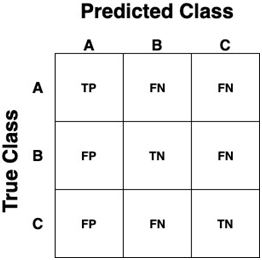
\includegraphics[scale=0.4]{multiclass_cfm}
	\caption{Multi-Class Confusion Matrix}
	\label{fig:figure6}
\end{figure}

\newpage

\subsection{Performance Metrics}

\begin{itemize}
	\item Test accuracy
	\begin{itemize}
		\item Measures how well the model makes correct predictions on data it has not seen before in training. $\frac{TP + TN}{TP + TN + FP + FN}$
	\end{itemize}
	\item Precision score
	\begin{itemize}
		\item Measures how many positive predictions are true positives. $\frac{TP}{TP + FP}$
	\end{itemize}
	\item Recall score
	\begin{itemize}
		\item Measures how well the model predicts all positive instances. $\frac{TP}{TP + FN}$
	\end{itemize}
	\item F1 score
	\begin{itemize}
		\item Measure the mean between precision and recall. $\frac{2 * Precision * Recall}{Precision + Recall}$
		\item This is especially useful since our dataset has a different amount of instances of each class. 
	\end{itemize}
\end{itemize}

\subsection{SVM}

SVM took a long time to run when looking at all the data, resulting in several days being taken to compute a single model.
By using Grid Search to find the best hyperparameter values, we were able to compute the following Confusion Matrix seen in Figure \ref{fig:figure7a}.
However, this model was severely overfitting as seen in Figure \ref{fig:figure7b}.
It was decided that instead of trying to work with SVM which would take a long time to compute the model, we would focus more on the various CNN algorithms.
The best hyperparameters found to compute the following results were $C = 10$ and $\gamma = \frac{1}{250,001}$.

\begin{figure}[h]
    \label{fig:figure7}
    \begin{subfigure}{0.4\textwidth}
        \centering
        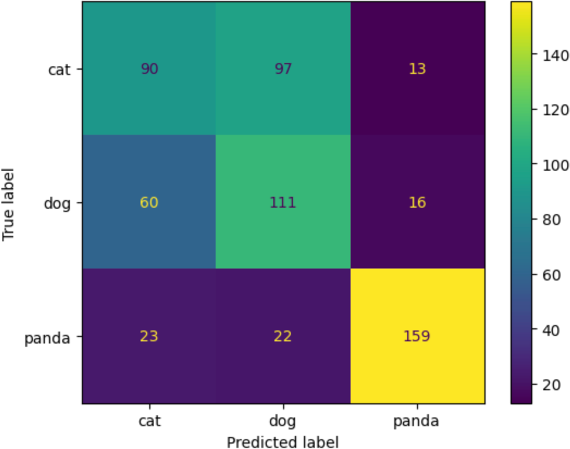
\includegraphics[scale=0.5]{csvm_cfm}
        \caption{Confusion Matrix of SVM}
        \label{fig:figure7a}
    \end{subfigure}
    \hspace{0.2\textwidth}
	\begin{subfigure}{0.4\textwidth}
        \centering
        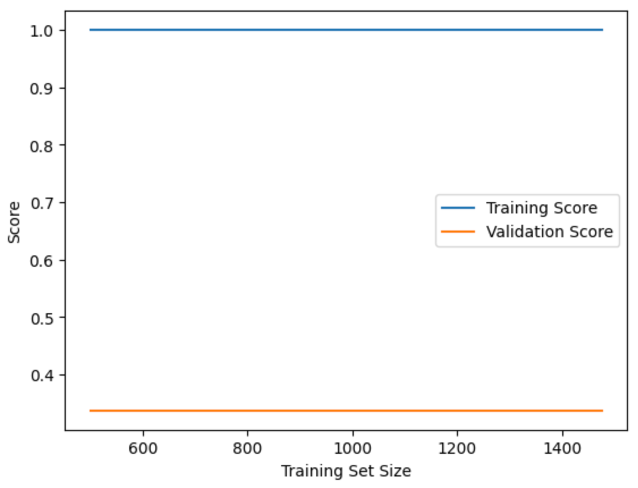
\includegraphics[scale=0.5]{svm_overfit}
        \caption{Loss function vs Training Size(Epochs) for SVM}
        \label{fig:figure7b}
    \end{subfigure}
\end{figure}

\subsection{CNN}
The first few training runs were done on a simpler CNN model with less convoluted and max-pooling layers. 
While run time was fairly quick, performance was low as the model was too simple. 
We experimented with adding more convoluted and max-pooling layers and found that adding too many made training time too long considering that performance did not improve much. 
The final structure is what we found to be the most efficient training-time wise for our project while also considering performance. 
Most runs averaged between 50-60\% accuracy before applying data augmentation and improved to 60-70\% after applying data augmentation. 
Our final run reached about 76\% test accuracy with a 76\% precision score, 76\% recall score, and a 75\% f1 score. 
The confusion matrix for our final CNN run is shown in Figure \ref{fig:figure8} below.
The model consistently had the most difficulty classifying dogs and the most success classifying pandas.

\begin{figure}[h]
	\centering
	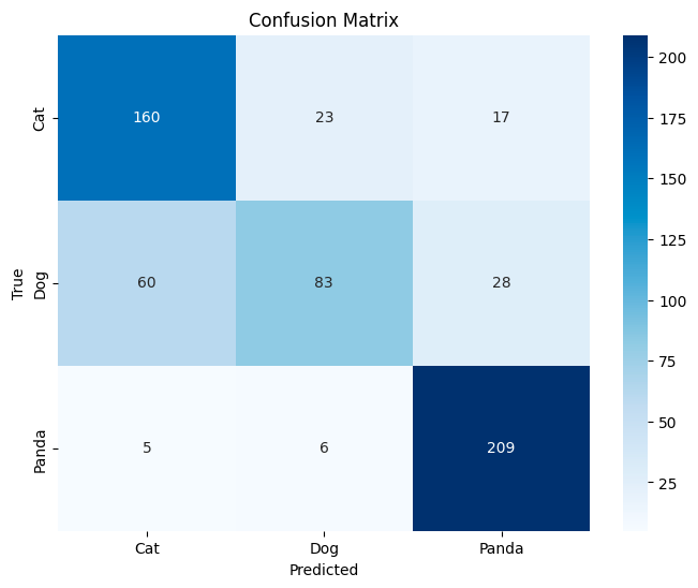
\includegraphics[scale=0.4]{CNN_cfm}
	\caption{Confusion matrix for final CNN run}
	\label{fig:figure8}
\end{figure}

\subsection{ResNet50}

There were several models that were made in order to get better results.
The structure of the networks used differing amounts of hidden layers, dropout, Conv2D, and MaxPooling2D layers in order to find the best performing model.
Ultimately, it was reduced to modifying 2 structures and having a basic model that would be the baseline to compare to.
We found that the best perfoming model was a simple structure with a single hidden layer with a dropout of 20\%, i.e. the baseline.
This model yielded an accuracy of 61\%, and showed strong signs of learning without overfitting nor underfitting seen in Figures \ref{fig:figure9a} and \ref{fig:figure9b}.


\begin{figure}[h]
    \begin{subfigure}{0.4\textwidth}
        \centering
        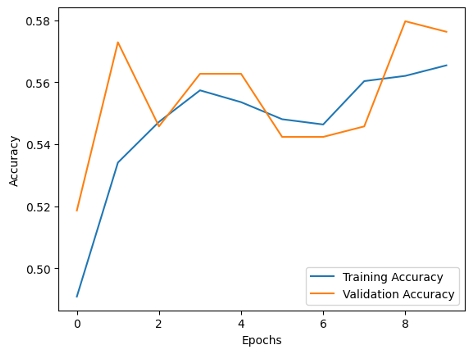
\includegraphics[scale=0.5]{resnet50_acc}
        \caption{Res Net 50: Accuracy vs Epochs}
        \label{fig:figure9a}
    \end{subfigure}
    \hspace{0.2\textwidth}
    \begin{subfigure}{0.4\textwidth}
        \centering
        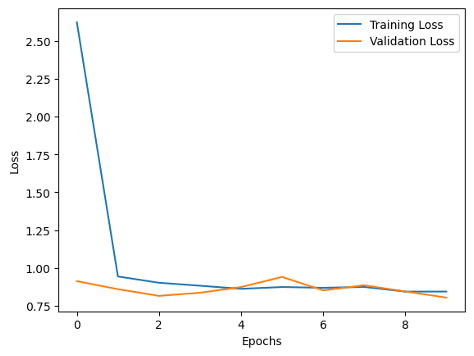
\includegraphics[scale=0.5]{resnet50loss}
        \caption{Res Net 50: Loss vs Epochs}
        \label{fig:figure9b}
    \end{subfigure}
\end{figure}

\subsection{VGG16}
The first training run was done with 3 dense layers manually added on top of the pre-trained VGG16 model and took approximately 14 hours to run through 15 epochs (there were 25 total epochs but the EarlyStopping callback was implemented which stopped training after 15 epochs). 
This first run yielded about 50\% accuracy and after experimenting with different hyperparameter values, it was apparent that the long run time could be shortened by removing a dense layer to decrease the complexity of the model without sacrificing performance too much. 
This is most likely because our dataset is small compared to what the VGG16 model was pre-trained on, and so an increase in complexity did not increase performance as the model struggled learn stably. 
Reducing the number of dense layers to 2 decreased training time to approximately 18 minutes per epoch (as opposed to 1 hour and 20 minutes per epoch before removing the third dense layer). 
Most runs stayed between 50-60\% with and without data augmentation. 
Our final run scored about 55\% on test accuracy, 58\% on precision, 55\% on recall, and 49\% on f1. 
The confusion matrix for our final VGG16 run is shown in Figure\ref{fig:figure10} below, where a significant number of false predictions can be observed. 

\begin{figure}[h]
	\centering
	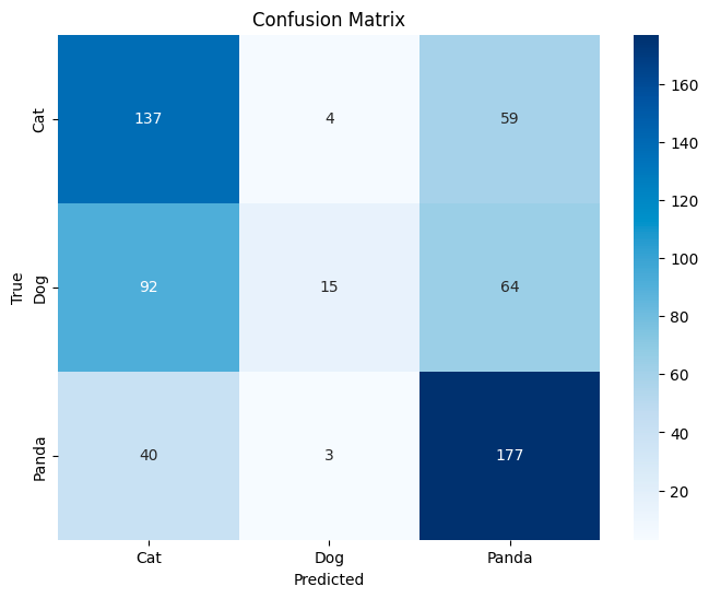
\includegraphics[scale=0.4]{VGG16_cfm}
	\caption{Confusion matrix for final VGG16 run.}
	\label{fig:figure10}
\end{figure}